In this section, we will derive preliminary results on our definition of security. We will first show implications between previous notions and relate those notions to our notion. We will then show how to compute the expectation of our security game by considering the idealised counterpart.


\subsection{Implications between Previous Notions}
We will show later that in order to bound the expectation in our security game, the scheme need to be secure in the black-box model. By that we mean the scheme has to satisfy semantic security of \cite{CCS:CGKO06} with the order of quantifiers reversed, i.e. there exists a simulator that works for all adversaries. Black-box model appears in \cite{FC:KurOht12}, and all proofs of schemes satisfying SS-CKA. For simplicity of notation, we prove relations with passive adversaries. All results can be converted to dynamic adversaries easily. We begin by giving definitions of the security notions.


\begin{definition}[Semantic Security Notion for Bit Adversaries]
	Consider the following game.
	
	\begin{pchstack}[center]
		\procedure{Real$_{\mathcal{\adv}}(n)$}{%
			\pcln \key \sample \kgen(\secparam) \\
			\pcln (\db, \stateA)  \gets \adv_0(\secparam) \\
			\pcln \edb, \gets \enc(\secparam, \key, \db) \\
			\pcln b \gets \adv_1(\secparam, \edb, \stateA) \\
			\pcln \pcreturn b
		}	
		
		\pchspace
		\procedure{$\simulator_{\mathcal{\adv,S}}(n)$}{%
			\pcln (\db, \stateA)   \gets \adv_0(\secparam) \\
			\pcln \leak \gets \leakm(\secparam, \db) \\
			\pcln \edb  \gets \mathcal{S}(\secparam, \leak) \\
			\pcln b \gets \adv_1(\secparam, \edb, \stateA) \\
			\pcln \pcreturn b
		}
	\end{pchstack}
	
	We say that the underlying searchable encryption scheme is $\leakm$-semantic secure in the black-box model for bit adversary if there exists a simulator $\mathcal{S}$ such that for all PPT adversaries $\adv = (\adv_0, \adv_1)$ where $\adv_1$ outputs a bit,
	\begin{equation}
	\prob{\text{Real}_\adv(n) = 1} - \prob{\simulator_\mathcal{\adv,S}(n) = 1} \leq \negl.
	\end{equation}
	
	We say that the underlying searchable encryption scheme is $\leakm$-semantic secure in the non-black-box model for bit adversary if for all PPT adversaries $\adv = (\adv_0, \adv_1)$ where $\adv_1$ outputs a bit, there exists a simulator $\mathcal{S}$ such that,
	\begin{equation}
	\prob{\text{Real}_\adv(n) = 1} - \prob{\simulator_\mathcal{\adv,S}(n) = 1} \leq \negl.
	\end{equation}
\end{definition}


\begin{definition}[Semantic Security Notion for String Adversaries]
	Consider the following game.
	
	\begin{pchstack}[center]
		\procedure{Real$_{\mathcal{\adv}}(n)$}{%
			\pcln \key \sample \kgen(\secparam) \\
			\pcln (\db, \stateA)  \gets \adv_0(\secparam) \\
			\pcln \edb, \gets \enc(\secparam, \key, \db) \\
			\pcln s \gets \adv_1(\secparam, \edb, \stateA) \\
			\pcln \pcreturn s
		}	
		
		\pchspace
		\procedure{$\simulator_{\mathcal{\adv,S}}(n)$}{%
			\pcln (\db, \stateA)   \gets \adv_0(\secparam) \\
			\pcln \leak \gets \leakm(\secparam, \db) \\
			\pcln \edb  \gets \mathcal{S}(\secparam, \leak) \\
			\pcln s \gets \adv_1(\secparam, \edb, \stateA) \\
			\pcln \pcreturn s
		}
	\end{pchstack}
	
	We say that the underlying searchable encryption scheme is $\leakm$-semantic secure in the black-box model for string adversary if there exists a simulator $\mathcal{S}$ such that for all PPT adversaries $\adv = (\adv_0, \adv_1)$, for all PPT distinguishers $\dister$, 
	\begin{equation}
	\prob{\dister(\text{Real}_\mathcal{A}(n)) = 1} - \prob{\dister(\simulator_\mathcal{A,S}(n)) = 1} \leq \negl.
	\end{equation}
	
	We say that the underlying searchable encryption scheme is $\leakm$-semantic secure in the non-black-box model for string adversary if for all PPT adversaries $\adv = (\adv_0, \adv_1)$, there exists a simulator $\simer$, such that for all PPT distinguishers $\dister$, 
	\begin{equation}
	\prob{\dister(\text{Real}_\mathcal{A}(n)) = 1} - \prob{\dister(\simer_\mathcal{A,S}(n)) = 1} \leq \negl.
	\end{equation}
	
\end{definition}

For simplicity, we call the four notions \textbf{B-BB-SS}, \textbf{B-NBB-SS}, \textbf{S-BB-SS} and \textbf{S-NBB-SS} respectively. We will now present the implications.

\begin{figure}[H]
	\centering
	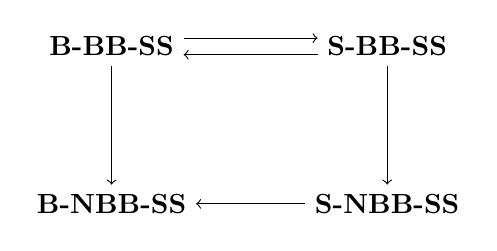
\begin{tikzpicture}[node distance=3.5cm, auto]
	\node (1) {\textbf{B-BB-SS}};
	\node (2) [below of=1, node distance=2cm] {\textbf{B-NBB-SS}};
	\node (3) [right of=1]{\textbf{S-BB-SS}};
	\node (4) [below of=3, node distance=2cm] {\textbf{S-NBB-SS}};
	
	\draw[->] (1) to (2);
	\draw[->] (3) to (4);
	\draw[->] (4) to (2);
	\draw[->,transform canvas={yshift=0.3em}] (1) to (3);
	\draw[->,transform canvas={yshift=-0.3em}] (3) to (1);
	\end{tikzpicture}
	\caption{Implication between notions}
\end{figure}

To summarise the implications, we have:
\begin{enumerate}
	\item In the black-box model, bit adversary and string adversary are equally strong.
	\item Security in black-box model implies security in non-black-box model.
	\item In the non-black-box model, bit adversary and string adversary are not equivalent.
\end{enumerate}

We will now give a proof of the implications.

\begin{proof}
	To begin with, we show that security in black-box model implies security in non-black-box model. Suppose there is a bit adversary in the black-box model, then this adversary works for all simulators, hence by using this adversary in the non-black box model, he wins with probability equal to the amount he wins in the black-box model. Hence for bit adversaries, security in black-box model implies security in non-black-box model. We use a very similar argument for string adversaries, the only difference is that we use the $(\adv, \dister)$ that breaks the security in the black-box model to break security in the non-black-box model.
	
	Since bit adversary is a special type of string adversary, we have implications from string adversary to bit adversary for free. It remains to show that in the black-box model, security against bit adversary implies security against string adversary. Suppose that the scheme is not secure against string adversary, then for all simulators, there exists an adversary $\adv$ such that there is a distinguisher $\dister$ wining the security game with non-negligible probability. The bit adversary can be easily constructed by composing $\adv$ and $\dister$, i.e. we run the two adversaries one after another and returns the bit from $\dister$ as the answer of the bit adversary. The bit adversary wins with probability equal to that of the corresponding string adversary. 
\end{proof}



